\chapter{Experimental Study of Spectral Clustering Techniques}
\label{Chapter4}

In this chapter we aim to study the effect of different relaxation methods (see ch.~\ref{SpectRelax}) applied to video segmentation. 
For evaluation of the video segmentation results we first introduce the boundary and volume oriented metric of~\cite{Galasso13}.

We then continue with a number of experiments comparing the performance of two relaxation techniques of the balanced graph cut problem - spectral clustering and 1-spectral clustering.
To make the comparison fair, we use an identical setting for both methods. The results are tested on the BMDS (see sec.~\ref{sec:ch3_dataset}). 

Finally, in order to analyze the behaviour of different balanced cut criteria and the solution produced by mentioned above methods we conducted several experiments with the ground truth. We tried to find a better partition by 
a trivial greedy search optimizing different objective functions: NCut, RCut, NCC, RCC, MinMaxCut and Cut (see sec.~\ref{sec:ch2_balgrcut}) and see if the optimal in the sense of balanced graph cuts solution is coincides with the 
human annotated segmentation.  
%%
% \section{Spectral Methods for Video Segmentation}
% \label{ch4:recap}
% In the proposed video segmentation model (see sec.~\ref{sec:ch3_framework}) first the graph is constructed on pre-computed superpixels and then the spectral method is applied to obtain the final segmentation. 
% In this work we consider two relaxation techniques of balanced graph cuts: spectral clustering (see sec.~\ref{sec:ch2_spectclus}) 
% and 1-spectral clustering (see sec.~\ref{sec:ch2_1spectclus}).
% 
% The standard 2-norm approach leads to a linear eigenproblem for the graph Laplacian, where the second eigenvector of the graph Laplacian corresponds to relaxation of the balanced graph cut.
% Spectral clustering has proved to be successful in segmentation. However, it is known to be loose and may yield solutions far from the optimal one.
% 1-spectral clustering gives a tight relaxation and in practice provides much better graph cuts than standard spectral clustering approach.
% This relaxation leads to a non-linear eigenproblem for the graph 1-Laplacian and the method does not guarantee convergence to the global optimum.
% 
% In contrast to spectral clustering, in 1-spectral clustering for multipartitioning the sequential splitting procedure with thresholding of the second eigenvector of the 1-Laplacian is used.
% Like for the 2-norm relaxation applying k-means here is not possible, as at the moment computation of higher-order eigenvectors of the 1-Laplacian is not feasible.
% 
% Both methods can optimize different balanced graph cut objectives (see sec.~\ref{sec:ch2_balgrcut}). However, the NCut is recommended itself by showing the state-of-the-art performance in image and video segmentation.
% In the experiments we consider normalized and unnormalized spectral clustering, which relaxes the NCut and RCut respectively. 
% Concerning 1-spectral clustering we use the following multipartition criteria: NCut, RCut, NCC and RCC.
% 
% For all the experiments for 1-spectral clustering the MATLAB implementation by~\cite{Buhler09} was used. The source code can be found at
% \url{http://www.ml.uni-saarland.de/code/oneSpectralClustering/1SpectralClustering_V1_1.rar}.
%In this section our goal is to investigate the benefits and shortcomings of employing different relaxation methods in video segmentation. 
\section{Evaluation Benchmark for Video Segmentation}
\label{ch4:bench}
In order to examine video segmentation results of different spectral methods we first need to choose a metric that could deal with segmentation hierarchies and reflect the tradeoff between over-segmentation and segmentation accuracy.

Recently it was proposed by~\cite{Galasso13} to evaluate video segmentation performance with a boundary and volume oriented metrics against human ground-truth.  
This new benchmark can evaluate under- and over-segmentation and also takes into account temporal consistency of the segmentation. 
\subsection{Boundary precision-recall (BPR)}
The boundary-based evaluation metric developed by~\cite{Martin01,Arbelaez11} on the Berkeley segmentation dataset (BSDS) has become a standard for image segmentation. It estimates the quality of a segmentation boundary map
in the precision-recall framework. Precision measures the fraction of true positives in the produced contours and recall the fraction of ground truth boundary pixels detected:
\begin{equation*}
\begin{aligned}
 P=\frac{ \lvert S\bigcap \bigr ( \bigcup_{i=1}^M G_i \bigl ) \rvert}{\rvert S \lvert},\\
 R =\frac{ \sum_{i=1}^M \lvert S\bigcap G_i \rvert}{\sum_{i=1}^M\rvert G_i \lvert},
\end{aligned}
\end{equation*}
where $S$ is the computer generated boundary map and $\{ G_i\}_{i=1}^M$ are the sets of ground-truth boundaries.
To estimate the total performance the global F-measure is defined as the harmonic mean of precision and recall:
\begin{equation*}
 F = \frac{2PR}{P+R}.
\end{equation*}

The main limitation of this metric is that it evaluates every frame independently and does not consider consistency of segmentation across frames. Although it estimates the localization accuracy of segmentation boundaries quite well,
the methodology that directly measures the quality of segments is desirable. Therefore the following volume-based metric is considered.
\subsection{Volume precision-recall (VPR)}
The volume metric developed by~\cite{Galasso13} measures the spatio-temporal overlap between the machine generated segmentation $S$ and the human annotated segmentations $\{ G_i\}_{i=1}^M$. 
To avoid high scores with this metric for over- and under-segmentation (every pixel being a separate segment or a single segment for the whole video sequence) a lower bounds are subtracted from the overlap score: 
\begin{equation*}
\begin{aligned}
 P=\frac{ \sum_{i=1}^M \bigl [ \{ \sum_{s\in S} \max_{g \in G_i} \lvert s \bigcap g \rvert\} - \max_{g \in G_i} \rvert g\lvert \bigr ]}{M\rvert S \lvert - \sum_{i=1}^M \max_{g \in G_i}},\\
\qquad
\quad
 R =\frac{ \sum_{i=1}^M  \sum_{g\in G_i} \{\max_{s \in S} \lvert s\bigcap g \rvert-1 \}}{\sum_{i=1}^M \{ \rvert G_i \lvert - \Gamma_{G_i} \}},
\end{aligned}
\end{equation*}
where $\Gamma_{G_i}$ is the number of volumes in the ground truth $G_i$.

For both BPR and VPR  3 different quantities are reported: the Optimal Dataset Scale (ODS) - the best F-measure on the dataset for a fixed scale, the Optimal Segmentation Scale (OSS) - the aggregate F-measure over the dataset for 
the best scale and the Average Precision (AP) on full recall range - the area under the precision-recall curve. %All precision-recall curves in the experiments are obtained by hierarchical clustering

For comparison we also consider different complementary region-based metrics: the Variation of Information (VI)~\cite{Meila05}, which measures the distance between two segmentations in terms of their average conditional entropy and mutual information, the 
Probabilistic Rand Index (PRI)~\cite{rand1971, UnnikrishnanPH07}, which counts the number of pixel pairs which labels are consistent between the machine generated and human annotated segmentations, and the Segmentation Covering (SG)
~\cite{Arbelaez09}, which estimates the best possible covering of the ground truth by segments.  

The benchmark code proposed by~\cite{Galasso13} can be found at  \url{http://www.mpi-inf.mpg.de/~galasso/files/Benchmark.zip}.
\section{Experiments on 1-Spectral Clustering vs Spectral Clustering}
\label{sec:ch4_1sc_vs_sc}
In this section our goal is to investigate the benefits and shortcomings of employing different relaxation methods in video segmentation. Here we consider two techniques: spectral clustering (see sec.~\ref{sec:ch2_spectclus}) 
and 1-spectral clustering (see sec.~\ref{sec:ch2_1spectclus}). 2-norm relaxation has proved to be successful in segmentation, but may yield solutions far from the optimal one. 
Theoretically, 1-spectral clustering gives a tight relaxation, which should lead to a better solution than standard spectral clustering approach. 
Even though, it does not guarantee convergence to the global optimum.
Both methods can optimize different objective functions. However, the NCut is recommended itself by showing the state-of-the-art performance in image and video segmentation.

In our setup we consider normalized and unnormalized spectral clustering, which relaxes the NCut and RCut respectively. 
Concerning 1-spectral clustering we use the following multipartition criteria: NCut, RCut, NCC and RCC.

Due to the fact that in video segmentation we deal with superpixels in order to reduce computational complexity, in the balancing term of the ratio cuts the cardinality of cluster could be understood in two ways.
Originally by the cardinality we consider the number of vertices in the cluster, which is in our work the number of superpixels. This could lead to very unbalanced clusters as the actual size of
superpixels may vary significantly, for instance for the video sequence ``Marple4`` from 4 to 8203 pixels. To avoid this potential problem and strengthen the balancing term we suggest to understand by the size of clusters 
the actual number of pixels.
Therefore, in our experiments for 1-norm relaxation we distinguish the ratio cut and the ratio Cheeger cut balanced by the number and the actual size of superpixels. 
   
As a first step we directly apply our proposed video segmentation model, in which to obtain the final segmentation we use 1-norm and 2-norm relaxations with different cut criteria.
For all the experiments with 1-spectral clustering the MATLAB implementation by~\cite{Buhler09} was used. The source code can be found at
\url{http://www.ml.uni-saarland.de/code/oneSpectralClustering/1SpectralClustering_V1_1.rar}.

Figure~\ref{fig:seg_res} illustrates boundary and volume precision-recall curves (BPR and VPR respectively) on the BMDS for the suggested experimental settings. 
The curves are obtained by hierarchical clustering, 
starting from 2 till 600 clusters, where the top-left part of BPR and the down-right part of VPR corresponds to a small number of clusters. 
Numerical comparison is presented in Table~\ref{tab:sc_comparison}.
\begin{figure}[htbp]
\centering
\subfigure[BPR]{%
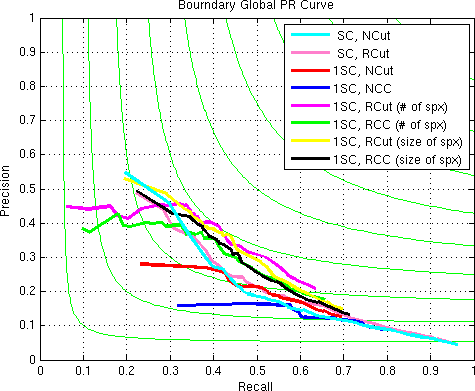
\includegraphics[trim=0cm 0cm 0cm 0.5cm, clip=true, width=0.41\textwidth]{images/basic/2.png}}
%\hfill
\quad
% \subfigure{%
% 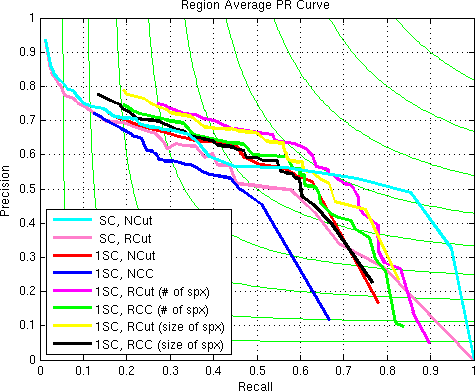
\includegraphics[trim=0cm 0cm 0cm 0.8cm, clip=true, width=0.47\textwidth]{images/basic/3.png}}
\subfigure[VPR]{%
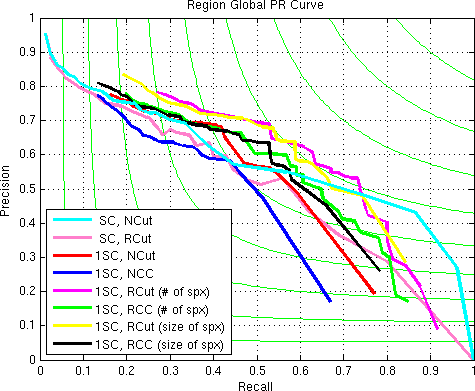
\includegraphics[trim=0cm 0cm 0cm 0.5cm, clip=true, width=0.41\textwidth]{images/basic/4.png}}

\caption[Boundary precision-recall (BPR) and volume precision-recall (VPR) curves for spectral clustering (SC) and 1-spectral clustering (1SC) with different cut criteria]{
{\bf Boundary precision-recall (BPR) and volume precision-recall (VPR) curves for spectral clustering (SC) and 1-spectral clustering (1SC) with different cut criteria.}}
\label{fig:seg_res}
\end{figure}

\begin{table}[htbp]
\renewcommand{\arraystretch}{1.3}
\centering
\scriptsize
%\sffamily
\begin{tabular}{|l||c|c|c||c|c|c||c|c|c||}
\hline 
\multirow{2}{*}{\textbf{Method}} & \multicolumn{3}{c||}{\textbf{BPR}} & \multicolumn{3}{c||}{\textbf{VPR}}& \multicolumn{3}{c||}{\textbf{Region}}\\
\cline{2-10}
& \textbf{ODS}  & \textbf{OSS} & \textbf{AP}
& \textbf{ODS} & \textbf{OSS} & \textbf{AP}
& \textbf{SC} & \textbf{PRI} & \textbf{VI} \\
\hline
\hline
\textbf{SC, NCut} & 0.36 & 0.39 & 0.21 & 0.59 &\textbf{0.72} & \textbf{0.59} & \textbf{0.89} & \textbf{0.78} & \textbf{0.67} \\
\hline
\textbf{SC, RCut} & 0.36 & 0.40 & 0.21 & 0.55 & 0.65 & 0.51 & 0.87 & 0.73 & \textbf{0.67} \\
\hline
\hline
\textbf{1SC, NCut} & 0.32 & 0.33 & 0.17 & 0.55 & 0.64 & 0.47 & 0.69 & 0.63 & 1.13 \\
\hline
\textbf{1SC, NCC} & 0.25 & 0.29 & 0.12 & 0.50 & 0.56 & 0.40 & 0.61 & 0.58 & 1.31 \\
\hline
\textbf{1SC, RCut (\# of spx)} &\textbf{0.40} & \textbf{0.45} & 0.25 & \textbf{0.62} & 0.69 & 0.58 & 0.82 & 0.70 & 0.86 \\
\hline
\textbf{1SC, RCC (\# of spx)} & 0.38 & 0.42 & 0.22 & 0.58 & 0.65 & 0.52 & 0.76 & 0.68 & 0.97 \\
\hline
\textbf{1SC, RCut (size of spx)} & \textbf{0.40} & \textbf{0.45} & \textbf{0.28} & 0.61 & 0.69 & 0.57 & 0.77 & 0.71 & 0.93 \\
\hline
\textbf{1SC, RCC (size of spx)} & 0.38 & 0.43 & 0.26 & 0.58 & 0.65 & 0.51 & 0.72 & 0.66 & 1.06 \\
\hline
\end{tabular}
 \caption{{\bf Comparison of spectral clustering (SC) and 1-spectral clustering (1SC) optimizing different cut criteria.} 
The table shows aggregate measures (ODS, OSS, AP) for boundary precision-recall (BPR), volume precision-recall (VPR) and 
includes region statistics (SC, PRI, VI).}
\label{tab:sc_comparison}
\end{table}
As it can be seen from the quantitative results normalized spectral clustering outperforms 1-norm relaxation despite its theoretical properties. The performance of the NCut and NCC for 1-spectral clustering is quite low,
especially for small number of clusters. Surprisingly the ratio cuts perform better than normalized ones. They improve upon standard spectral clustering in boundary metric and give comparable results in volume oriented metric, 
particularly for a bigger number of clusters. Our proposed for the RCut and RCC balancing by the size of superpixels enhance the results compared to the balancing by number of superpixels. 
The unnormalized spectral clustering yields comparable results with the normalized one in BPR, but performs poorly in VPR. 
\newpage
These quantitative results are supported by qualitative results. Figures~\ref{fig:seg_res_C1} and~\ref{fig:seg_res_M4} illustrate final segmentations for video sequences ''Cars1'' for 2 clusters and ``Marple4'' for 3 clusters.

It was observed that the RCut and RCC, normalized by the number of superpixels, have a tendency to disconnect one small superpixel in one of the frames and usually require more clusters
to obtain meaningful solution where objects are well distinguished. 
The standard spectral clustering and tight relaxation for the ratio cuts, balanced by the size of superpixels, usually provide comparable segmentation results, where the RCut is slightly better than the RCC . 
The NCut and NCC tend to separate the sequence into clusters of equal size by the horizontal or vertical line, which could be explained by the strong balancing term of the normalized cuts. This results in poor 
overall performance.
%\subsection{Qualitative results}
\begin{figure}[ht!]
\begin{minipage}[t]{1\textwidth}
 \centering
\hfill \hfill  \hfill
\footnotesize Frame 1
\hfill  \hfill
\footnotesize Frame 9
\hfill  \hfill
\footnotesize Frame 11
\hfill  \hfill
\footnotesize Frame 19
\hfill \hfill  \hfill
\end{minipage}
% 

\begin{minipage}[t]{1\textwidth}
\centering
\hfill \hfill  \hfill
 \subfigure{%
 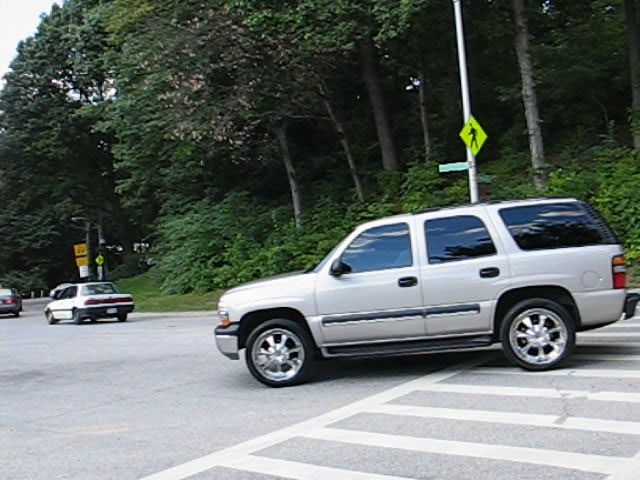
\includegraphics[width=0.16\textwidth]{images/pres/C1/cars1_01.jpg}}
\hfill
\subfigure{%
 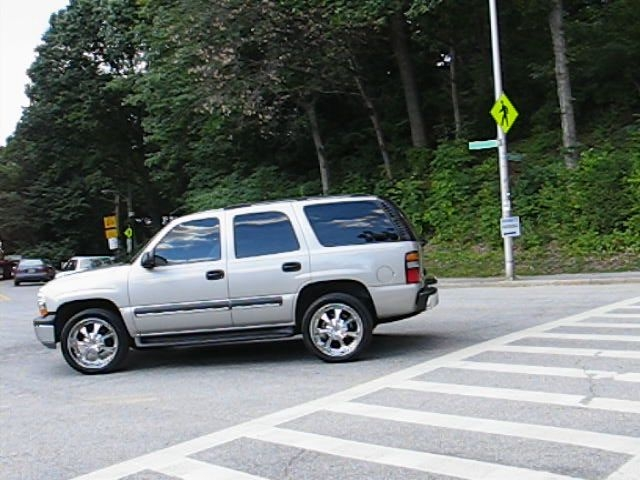
\includegraphics[width=0.16\textwidth]{images/pres/C1/cars1_09.jpg}}
\hfill
\subfigure{%
 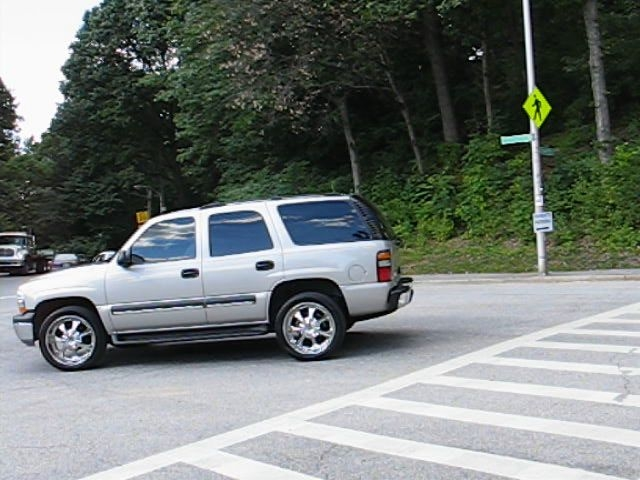
\includegraphics[width=0.16\textwidth]{images/pres/C1/cars1_11.jpg}}
\hfill
\subfigure{%
 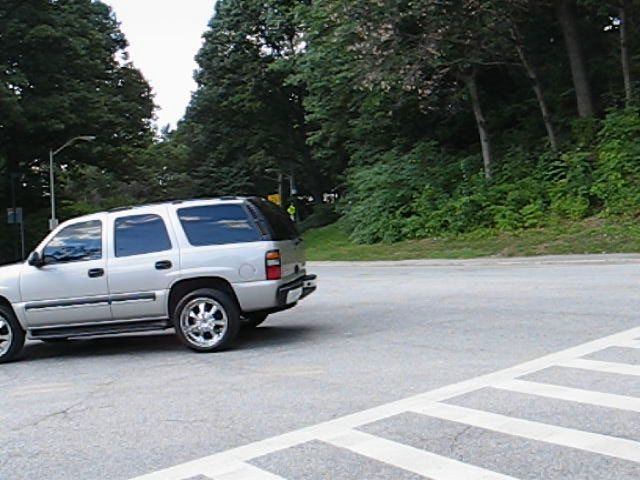
\includegraphics[width=0.16\textwidth]{images/pres/C1/cars1_19.jpg}}
\hfill \hfill  \hfill

\footnotesize (a) Marple4
\end{minipage}
\begin{minipage}[t]{1\textwidth}
\centering
\hfill \hfill  \hfill
 \subfigure{%
 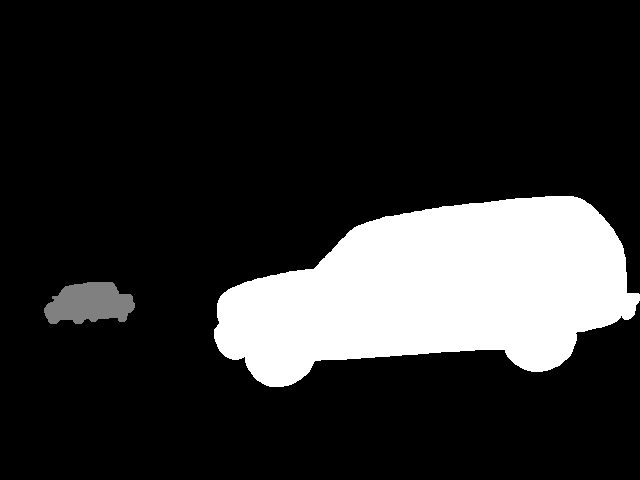
\includegraphics[width=0.16\textwidth]{images/pres/C1/cars1_01.png}}
\hfill
\subfigure{%
 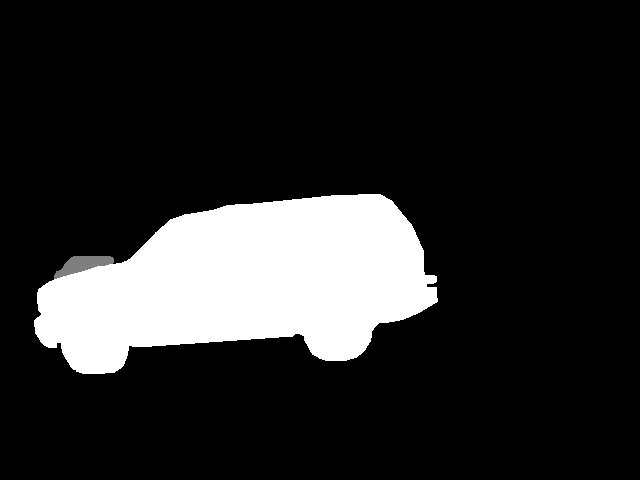
\includegraphics[width=0.16\textwidth]{images/pres/C1/cars1_09.png}}
\hfill
\subfigure{%
 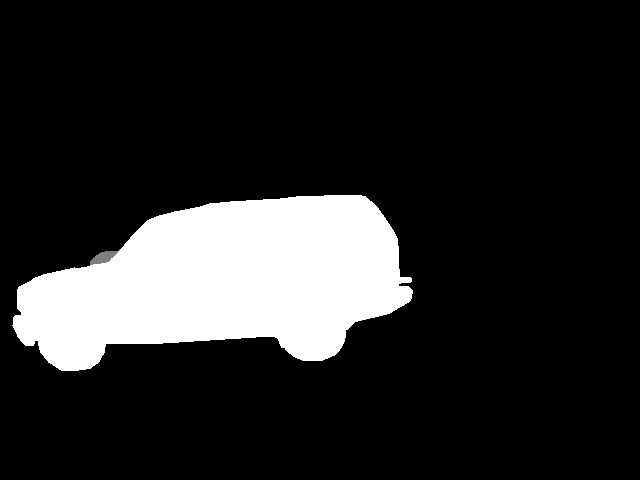
\includegraphics[width=0.16\textwidth]{images/pres/C1/cars1_11.png}}
\hfill
\subfigure{%
 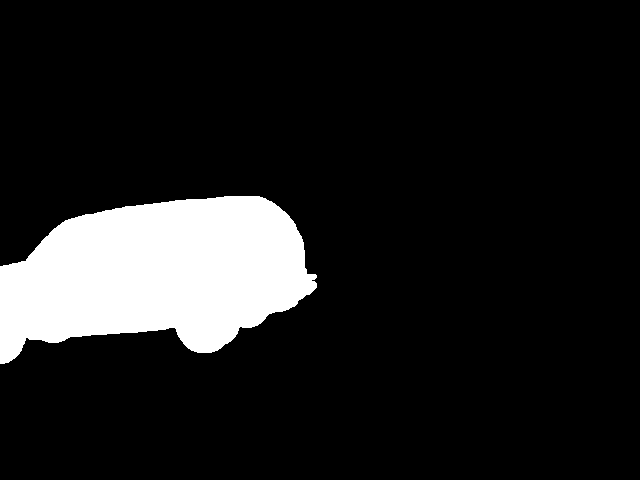
\includegraphics[width=0.16\textwidth]{images/pres/C1/cars1_19.png}}
\hfill \hfill  \hfill

\footnotesize (b) Ground Truth
\end{minipage}
\begin{minipage}[t]{1\textwidth}
\centering
\hfill \hfill  \hfill
 \subfigure{%
 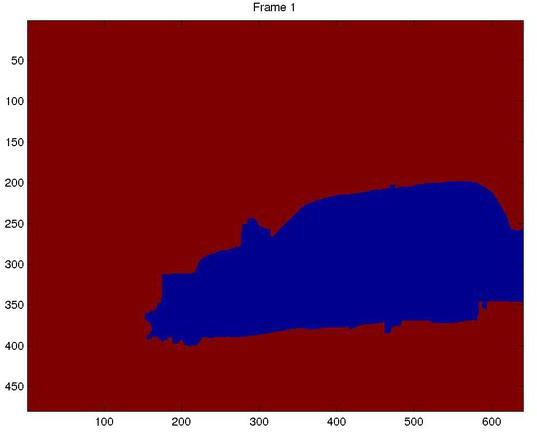
\includegraphics[trim=0cm 0cm 0cm 1cm, clip=true, width=0.17\textwidth]{images/pres/C1/sc/001.jpg}}
\hfill
\subfigure{%
 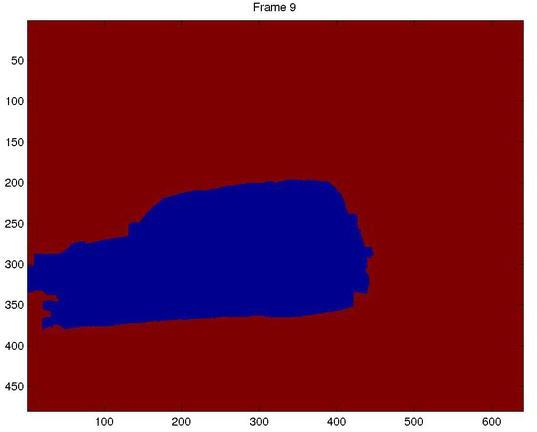
\includegraphics[trim=0cm 0cm 0cm 1cm, clip=true, width=0.17\textwidth]{images/pres/C1/sc/009.jpg}}
\hfill
\subfigure{%
 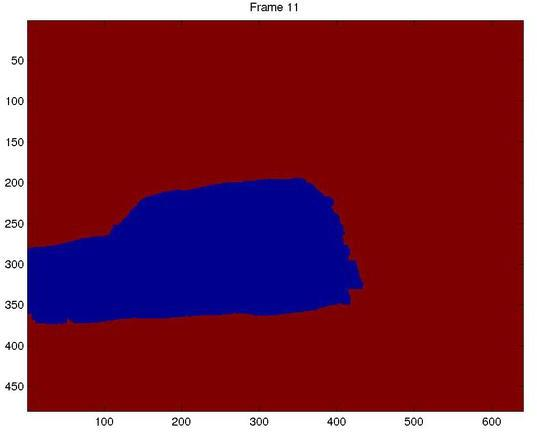
\includegraphics[trim=0cm 0cm 0cm 1cm, clip=true, width=0.17\textwidth]{images/pres/C1/sc/011.jpg}}
\hfill
\subfigure{%
 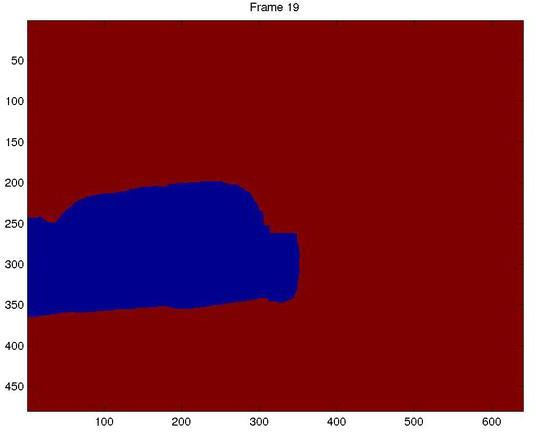
\includegraphics[trim=0cm 0cm 0cm 1cm, clip=true, width=0.17\textwidth]{images/pres/C1/sc/019.jpg}}
\hfill \hfill  \hfill

\footnotesize (c) Spectral Clustering
\end{minipage}
\begin{minipage}[t]{1\textwidth}
\centering
\hfill \hfill  \hfill
 \subfigure{%
 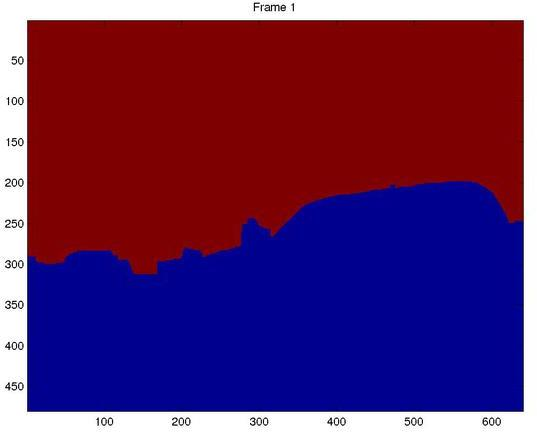
\includegraphics[trim=0cm 0cm 0cm 1cm, clip=true, width=0.17\textwidth]{images/pres/C1/ncut/001.jpg}}
\hfill
\subfigure{%
 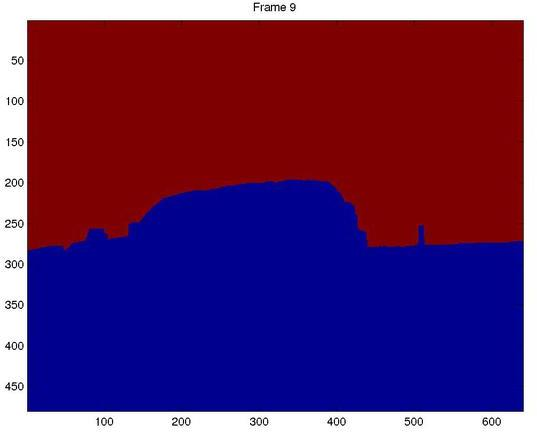
\includegraphics[trim=0cm 0cm 0cm 1cm, clip=true, width=0.17\textwidth]{images/pres/C1/ncut/009.jpg}}
\hfill
\subfigure{%
 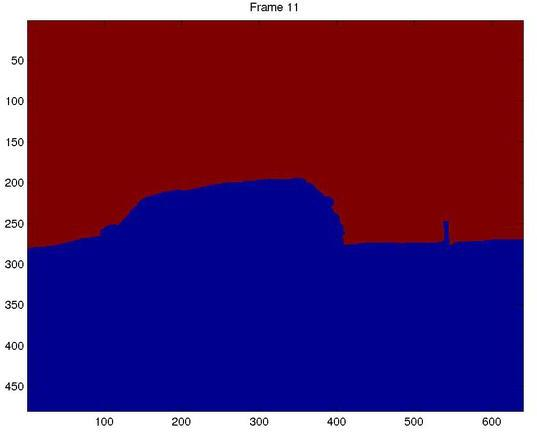
\includegraphics[trim=0cm 0cm 0cm 1cm, clip=true, width=0.17\textwidth]{images/pres/C1/ncut/011.jpg}}
\hfill
\subfigure{%
 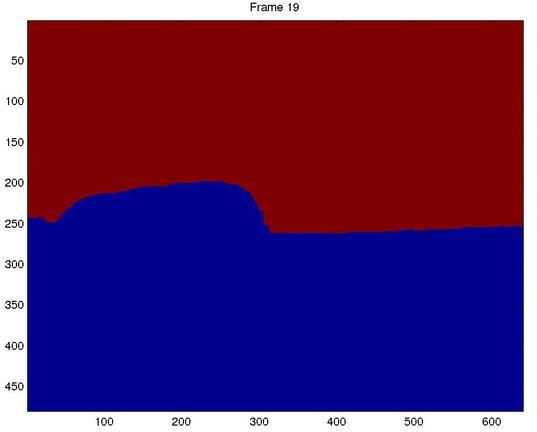
\includegraphics[trim=0cm 0cm 0cm 1cm, clip=true, width=0.17\textwidth]{images/pres/C1/ncut/019.jpg}}
\hfill \hfill  \hfill

\footnotesize (d) 1-Spectral Clustering, NCut
\end{minipage}
\begin{minipage}[t]{1\textwidth}
\centering
\hfill \hfill  \hfill
 \subfigure{%
 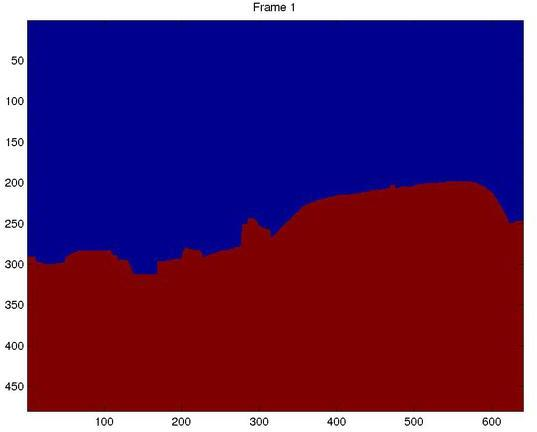
\includegraphics[trim=0cm 0cm 0cm 1cm, clip=true, width=0.17\textwidth]{images/pres/C1/ncc/001.jpg}}
\hfill
\subfigure{%
 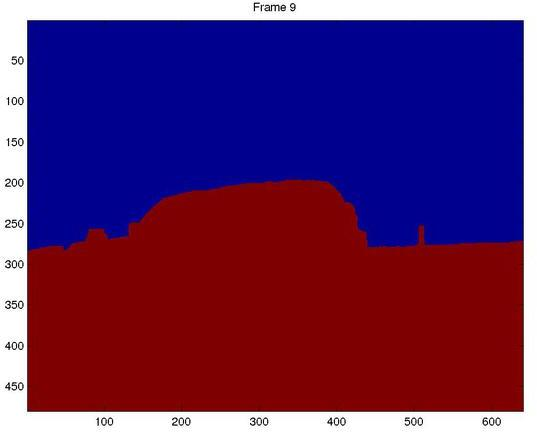
\includegraphics[trim=0cm 0cm 0cm 1cm, clip=true, width=0.17\textwidth]{images/pres/C1/ncc/009.jpg}}
\hfill
\subfigure{%
 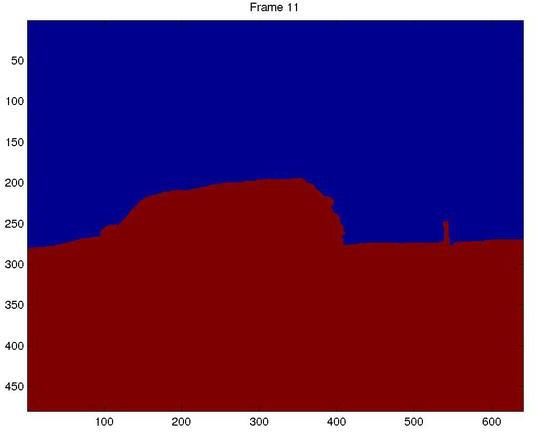
\includegraphics[trim=0cm 0cm 0cm 1cm, clip=true, width=0.17\textwidth]{images/pres/C1/ncc/011.jpg}}
\hfill
\subfigure{%
 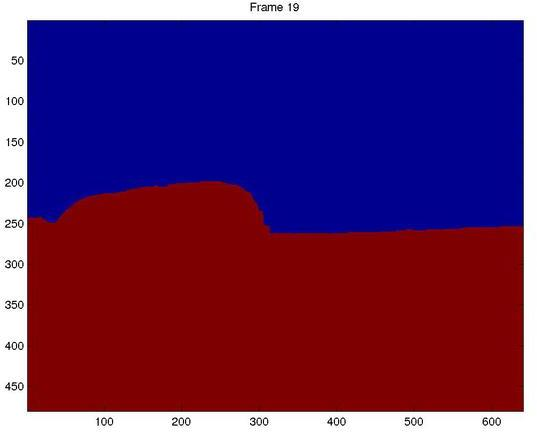
\includegraphics[trim=0cm 0cm 0cm 1cm, clip=true, width=0.17\textwidth]{images/pres/C1/ncc/019.jpg}}
\hfill \hfill  \hfill

\footnotesize (e) 1-Spectral Clustering, NCC
\end{minipage}
\begin{minipage}[t]{1\textwidth}
\centering
\hfill \hfill  \hfill
 \subfigure{%
 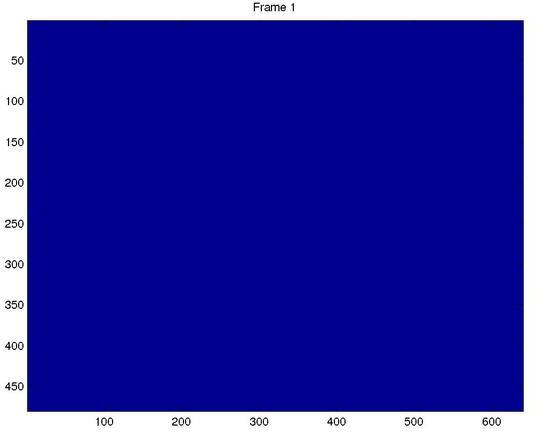
\includegraphics[trim=0cm 0cm 0cm 1cm, clip=true, width=0.17\textwidth]{images/pres/C1/rcut_old/001.jpg}}
\hfill
\subfigure{%
 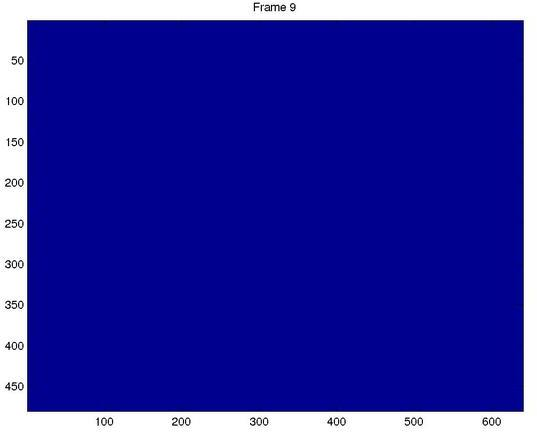
\includegraphics[trim=0cm 0cm 0cm 1cm, clip=true, width=0.17\textwidth]{images/pres/C1/rcut_old/009.jpg}}
\hfill
\subfigure{%
 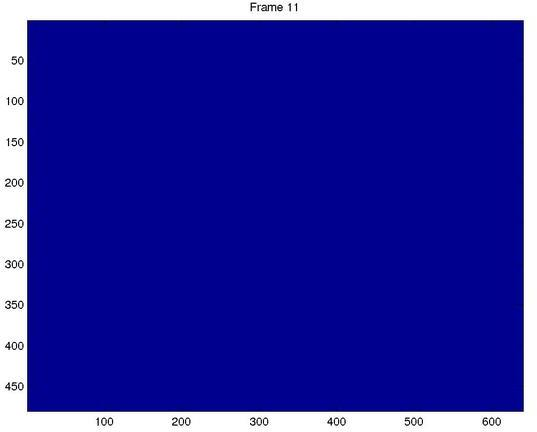
\includegraphics[trim=0cm 0cm 0cm 1cm, clip=true, width=0.17\textwidth]{images/pres/C1/rcut_old/011.jpg}}
\hfill
\subfigure{%
 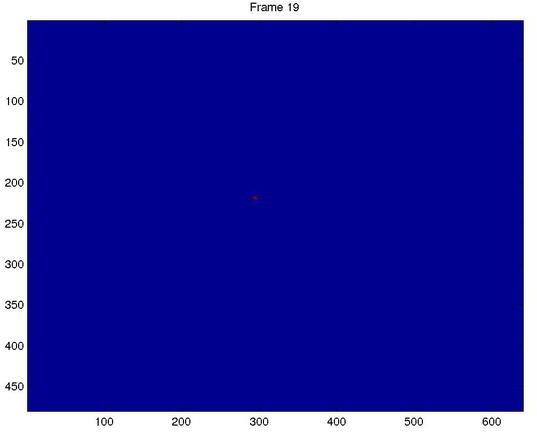
\includegraphics[trim=0cm 0cm 0cm 1cm, clip=true, width=0.17\textwidth]{images/pres/C1/rcut_old/019.jpg}}
\hfill \hfill  \hfill

\footnotesize (f) 1-Spectral Clustering, RCut (balanced by number of superpixels)
\end{minipage}
\begin{minipage}[t]{1\textwidth}
\centering
\hfill \hfill  \hfill
 \subfigure{%
 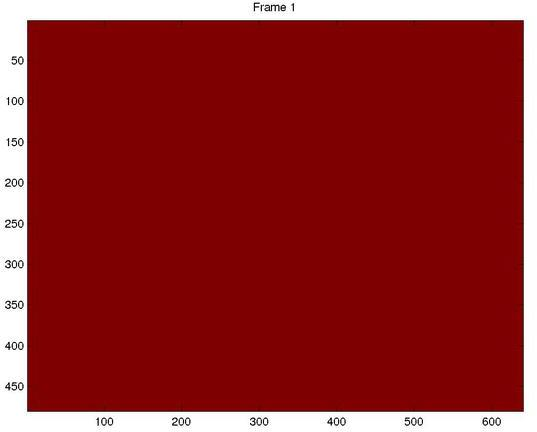
\includegraphics[trim=0cm 0cm 0cm 1cm, clip=true, width=0.17\textwidth]{images/pres/C1/rcc_old/001.jpg}}
\hfill
\subfigure{%
 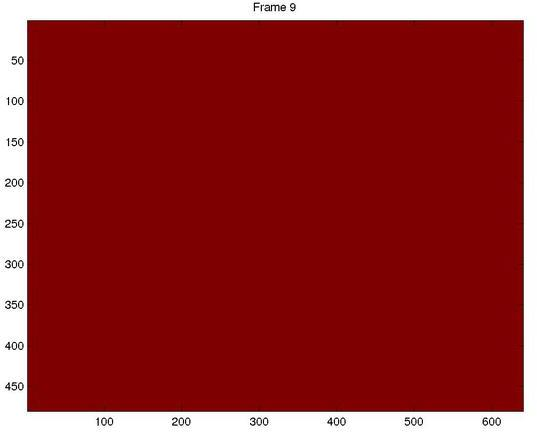
\includegraphics[trim=0cm 0cm 0cm 1cm, clip=true, width=0.17\textwidth]{images/pres/C1/rcc_old/009.jpg}}
\hfill
\subfigure{%
 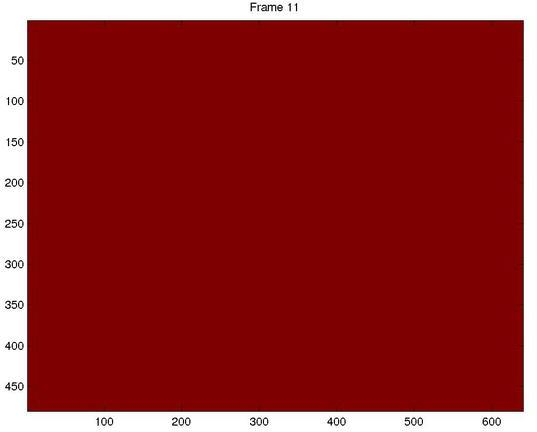
\includegraphics[trim=0cm 0cm 0cm 1cm, clip=true, width=0.17\textwidth]{images/pres/C1/rcc_old/011.jpg}}
\hfill
\subfigure{%
 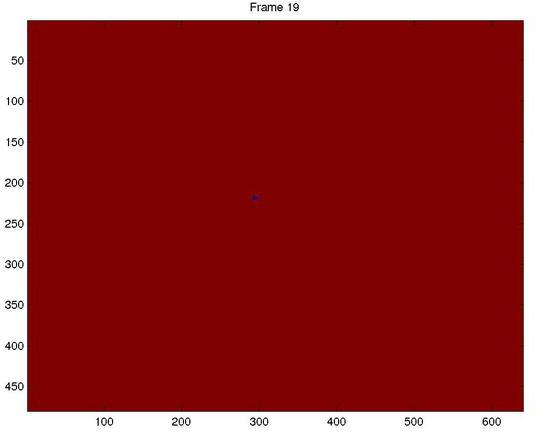
\includegraphics[trim=0cm 0cm 0cm 1cm, clip=true, width=0.17\textwidth]{images/pres/C1/rcc_old/019.jpg}}
\hfill \hfill  \hfill

\footnotesize (g) 1-Spectral Clustering, RCC (balanced by number of superpixels)
\end{minipage}
\begin{minipage}[t]{1\textwidth}
\centering
\hfill \hfill  \hfill
 \subfigure{%
 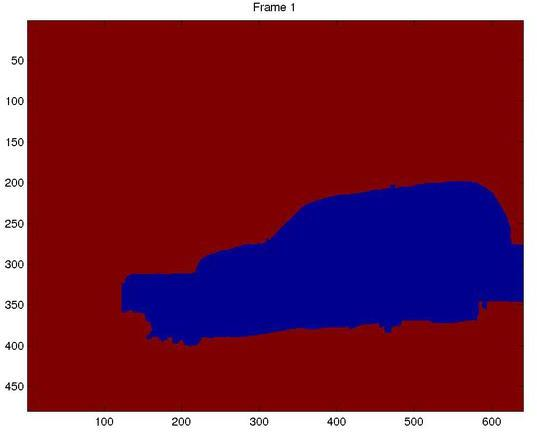
\includegraphics[trim=0cm 0cm 0cm 1cm, clip=true, width=0.17\textwidth]{images/pres/C1/rcut/001.jpg}}
\hfill
\subfigure{%
 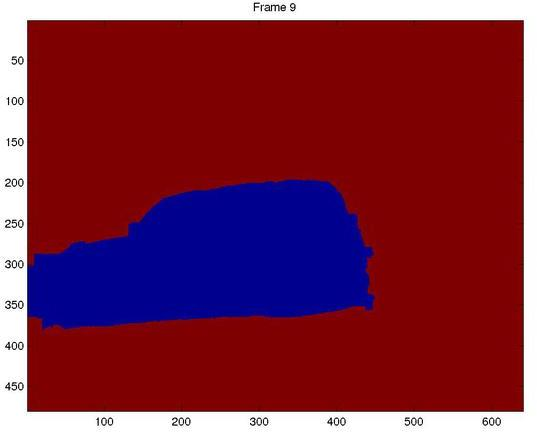
\includegraphics[trim=0cm 0cm 0cm 1cm, clip=true, width=0.17\textwidth]{images/pres/C1/rcut/009.jpg}}
\hfill
\subfigure{%
 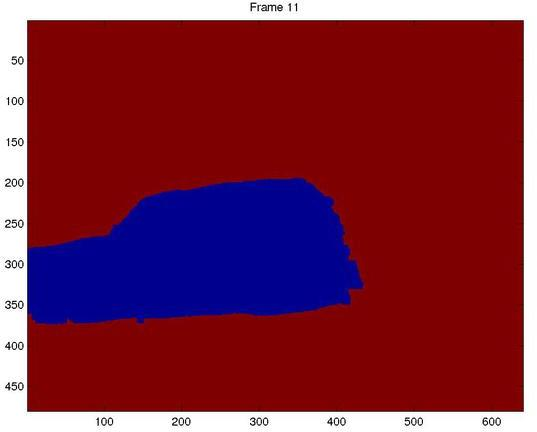
\includegraphics[trim=0cm 0cm 0cm 1cm, clip=true, width=0.17\textwidth]{images/pres/C1/rcut/011.jpg}}
\hfill
\subfigure{%
 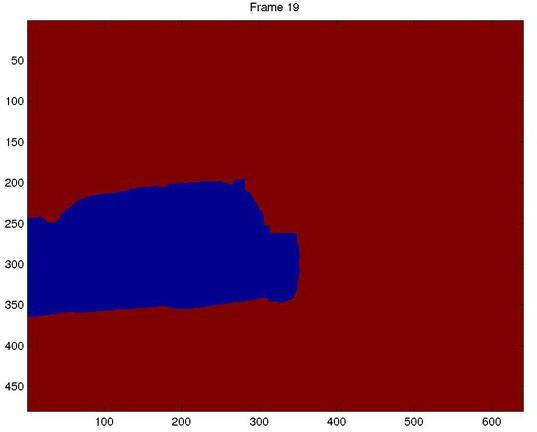
\includegraphics[trim=0cm 0cm 0cm 1cm, clip=true, width=0.17\textwidth]{images/pres/C1/rcut/019.jpg}}
\hfill \hfill  \hfill

\footnotesize (h) 1-Spectral Clustering, RCut (balanced by size of superpixels)
\end{minipage}
\begin{minipage}[t]{1\textwidth}
\centering
\hfill \hfill  \hfill
 \subfigure{%
 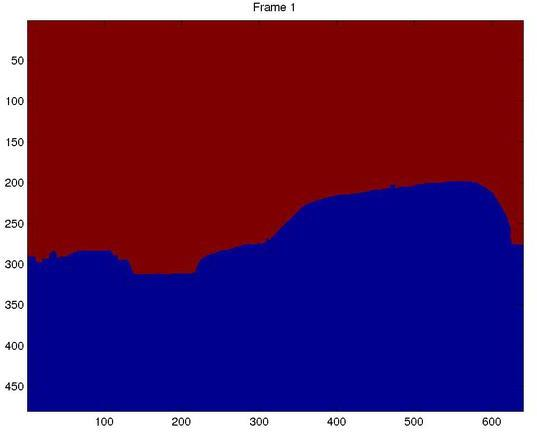
\includegraphics[trim=0cm 0cm 0cm 1cm, clip=true, width=0.17\textwidth]{images/pres/C1/rcc/001.jpg}}
\hfill
\subfigure{%
 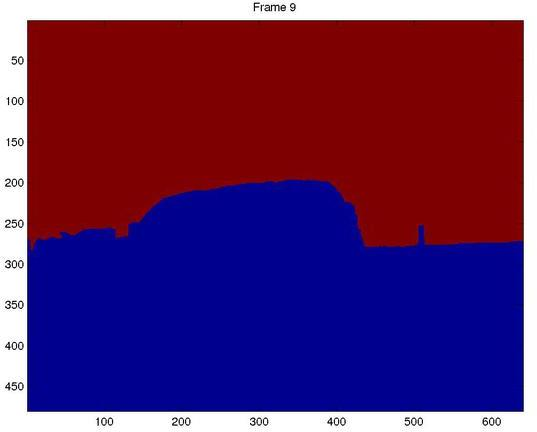
\includegraphics[trim=0cm 0cm 0cm 1cm, clip=true, width=0.17\textwidth]{images/pres/C1/rcc/009.jpg}}
\hfill
\subfigure{%
 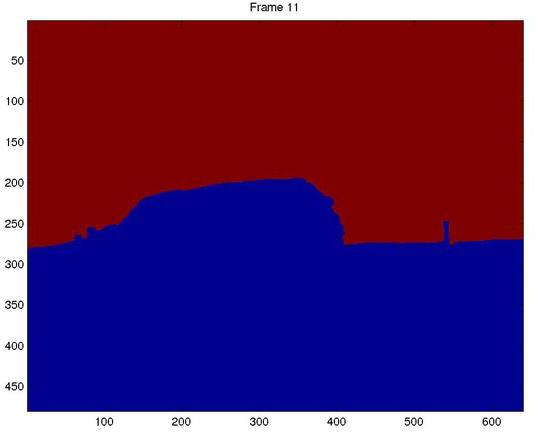
\includegraphics[trim=0cm 0cm 0cm 1cm, clip=true, width=0.17\textwidth]{images/pres/C1/rcc/011.jpg}}
\hfill
\subfigure{%
 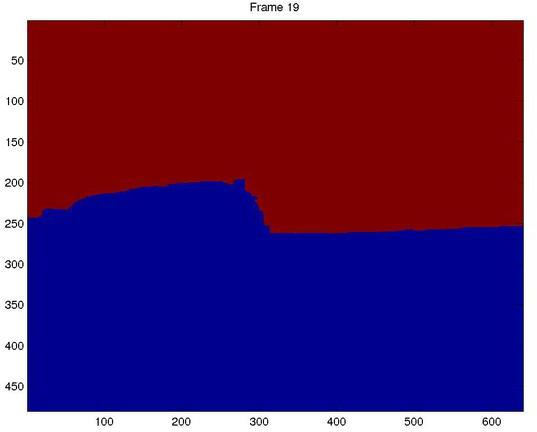
\includegraphics[trim=0cm 0cm 0cm 1cm, clip=true, width=0.17\textwidth]{images/pres/C1/rcc/019.jpg}}
\hfill \hfill  \hfill

\footnotesize (i) 1-Spectral Clustering, RCC (balanced by size of superpixels)
\end{minipage}
 \caption[Segmentation results for the video sequence ``Cars1`` for 2 clusters]{
  {\bf Segmentation results for the video sequence ``Cars1`` for 2 clusters.}}
\label{fig:seg_res_C1}
\end{figure}
\begin{figure}[ht!]
\begin{minipage}[t]{1\textwidth}
 \centering
\hfill \hfill  \hfill
\footnotesize Frame 1
\hfill  \hfill
\footnotesize Frame 10
\hfill  \hfill
\footnotesize Frame 20
\hfill  \hfill
\footnotesize Frame 30
\hfill \hfill  \hfill
\end{minipage}
% 

\begin{minipage}[t]{1\textwidth}
\centering
\hfill \hfill  \hfill
 \subfigure{%
 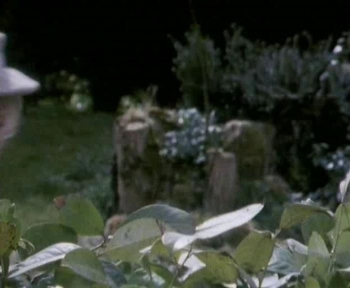
\includegraphics[width=0.16\textwidth]{images/pres/M4/marple4_324.jpg}}
\hfill
\subfigure{%
 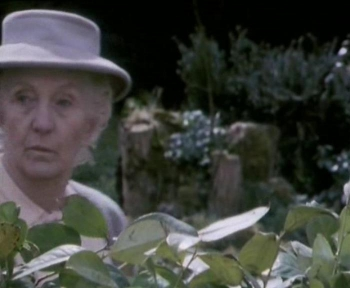
\includegraphics[width=0.16\textwidth]{images/pres/M4/marple4_333.jpg}}
\hfill
\subfigure{%
 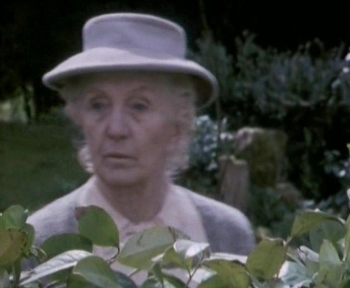
\includegraphics[width=0.16\textwidth]{images/pres/M4/marple4_343.jpg}}
\hfill
\subfigure{%
 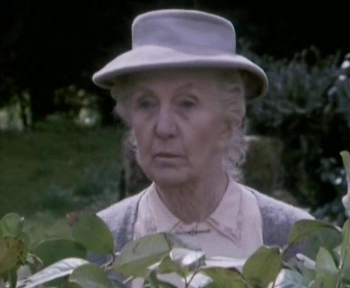
\includegraphics[width=0.16\textwidth]{images/pres/M4/marple4_353.jpg}}
\hfill \hfill  \hfill

\footnotesize (a) Marple4
\end{minipage}
\begin{minipage}[t]{1\textwidth}
\centering
\hfill \hfill  \hfill
 \subfigure{%
 
\includegraphics[width=0.16\textwidth]{images/pres/M4/marple4_324.png}}
\hfill
\subfigure{%
 
\includegraphics[width=0.16\textwidth]{images/pres/M4/marple4_333.png}}
\hfill
\subfigure{%
 
\includegraphics[width=0.16\textwidth]{images/pres/M4/marple4_343.png}}
\hfill
\subfigure{%
 
\includegraphics[width=0.16\textwidth]{images/pres/M4/marple4_353.png}}
\hfill \hfill  \hfill

\footnotesize (b) Ground Truth
\end{minipage}
\begin{minipage}[t]{1\textwidth}
\centering
\hfill \hfill  \hfill
 \subfigure{%
 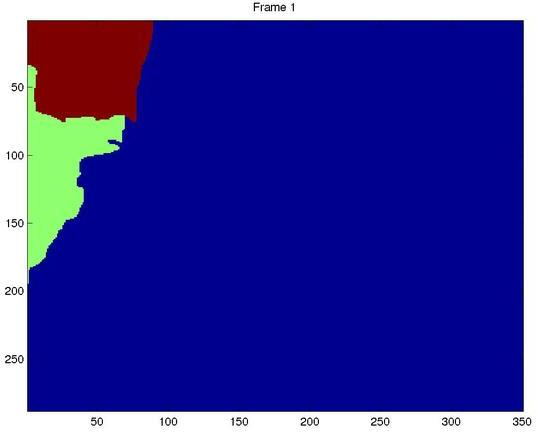
\includegraphics[trim=0cm 0cm 0cm 1cm, clip=true, width=0.17\textwidth]{images/pres/M4/sc/001.jpg}}
\hfill
\subfigure{%
 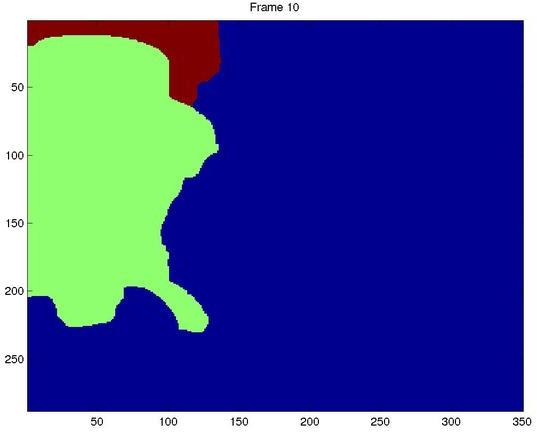
\includegraphics[trim=0cm 0cm 0cm 1cm, clip=true, width=0.17\textwidth]{images/pres/M4/sc/010.jpg}}
\hfill
\subfigure{%
 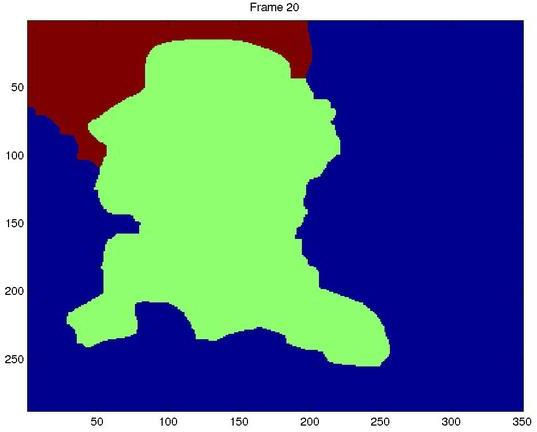
\includegraphics[trim=0cm 0cm 0cm 1cm, clip=true, width=0.17\textwidth]{images/pres/M4/sc/020.jpg}}
\hfill
\subfigure{%
 \includegraphics[trim=0cm 0cm 0cm 1cm, clip=true, width=0.17\textwidth]{images/pres/M4/sc/030.jpg}}
\hfill \hfill  \hfill

\footnotesize (c) Spectral Clustering
\end{minipage}
\begin{minipage}[t]{1\textwidth}
\centering
\hfill \hfill  \hfill
 \subfigure{%
 \includegraphics[trim=0cm 0cm 0cm 1cm, clip=true, width=0.17\textwidth]{images/pres/M4/ncut/001.jpg}}
\hfill
\subfigure{%
 \includegraphics[trim=0cm 0cm 0cm 1cm, clip=true, width=0.17\textwidth]{images/pres/M4/ncut/010.jpg}}
\hfill
\subfigure{%
 \includegraphics[trim=0cm 0cm 0cm 1cm, clip=true, width=0.17\textwidth]{images/pres/M4/ncut/020.jpg}}
\hfill
\subfigure{%
 \includegraphics[trim=0cm 0cm 0cm 1cm, clip=true, width=0.17\textwidth]{images/pres/M4/ncut/030.jpg}}
\hfill \hfill  \hfill

\footnotesize (d) 1-Spectral Clustering, NCut
\end{minipage}
\begin{minipage}[t]{1\textwidth}
\centering
\hfill \hfill  \hfill
 \subfigure{%
 \includegraphics[trim=0cm 0cm 0cm 1cm, clip=true, width=0.17\textwidth]{images/pres/M4/ncc/001.jpg}}
\hfill
\subfigure{%
 \includegraphics[trim=0cm 0cm 0cm 1cm, clip=true, width=0.17\textwidth]{images/pres/M4/ncc/010.jpg}}
\hfill
\subfigure{%
 \includegraphics[trim=0cm 0cm 0cm 1cm, clip=true, width=0.17\textwidth]{images/pres/M4/ncc/020.jpg}}
\hfill
\subfigure{%
 \includegraphics[trim=0cm 0cm 0cm 1cm, clip=true, width=0.17\textwidth]{images/pres/M4/ncc/030.jpg}}
\hfill \hfill  \hfill

\footnotesize (e) 1-Spectral Clustering, NCC
\end{minipage}
\begin{minipage}[t]{1\textwidth}
\centering
\hfill \hfill  \hfill
 \subfigure{%
 \includegraphics[trim=0cm 0cm 0cm 1cm, clip=true, width=0.17\textwidth]{images/pres/M4/rcut_old/001.jpg}}
\hfill
\subfigure{%
 \includegraphics[trim=0cm 0cm 0cm 1cm, clip=true, width=0.17\textwidth]{images/pres/M4/rcut_old/010.jpg}}
\hfill
\subfigure{%
 \includegraphics[trim=0cm 0cm 0cm 1cm, clip=true, width=0.17\textwidth]{images/pres/M4/rcut_old/020.jpg}}
\hfill
\subfigure{%
 \includegraphics[trim=0cm 0cm 0cm 1cm, clip=true, width=0.17\textwidth]{images/pres/M4/rcut_old/030.jpg}}
\hfill \hfill  \hfill

\footnotesize (f) 1-Spectral Clustering, RCut (balanced by number of superpixels)
\end{minipage}
\begin{minipage}[t]{1\textwidth}
\centering
\hfill \hfill  \hfill
 \subfigure{%
 \includegraphics[trim=0cm 0cm 0cm 1cm, clip=true, width=0.17\textwidth]{images/pres/M4/rcc_old/001.jpg}}
\hfill
\subfigure{%
 \includegraphics[trim=0cm 0cm 0cm 1cm, clip=true, width=0.17\textwidth]{images/pres/M4/rcc_old/010.jpg}}
\hfill
\subfigure{%
 \includegraphics[trim=0cm 0cm 0cm 1cm, clip=true, width=0.17\textwidth]{images/pres/M4/rcc_old/020.jpg}}
\hfill
\subfigure{%
 \includegraphics[trim=0cm 0cm 0cm 1cm, clip=true, width=0.17\textwidth]{images/pres/M4/rcc_old/030.jpg}}
\hfill \hfill  \hfill

\footnotesize (g) 1-Spectral Clustering, RCC (balanced by number of superpixels)
\end{minipage}
\begin{minipage}[t]{1\textwidth}
\centering
\hfill \hfill  \hfill
 \subfigure{%
 \includegraphics[trim=0cm 0cm 0cm 1cm, clip=true, width=0.17\textwidth]{images/pres/M4/rcut/001.jpg}}
\hfill
\subfigure{%
 \includegraphics[trim=0cm 0cm 0cm 1cm, clip=true, width=0.17\textwidth]{images/pres/M4/rcut/010.jpg}}
\hfill
\subfigure{%
 \includegraphics[trim=0cm 0cm 0cm 1cm, clip=true, width=0.17\textwidth]{images/pres/M4/rcut/020.jpg}}
\hfill
\subfigure{%
 \includegraphics[trim=0cm 0cm 0cm 1cm, clip=true, width=0.17\textwidth]{images/pres/M4/rcut/030.jpg}}
\hfill \hfill  \hfill

\footnotesize (h) 1-Spectral Clustering, RCut (balanced by size of superpixels)
\end{minipage}
\begin{minipage}[t]{1\textwidth}
\centering
\hfill \hfill  \hfill
 \subfigure{%
 \includegraphics[trim=0cm 0cm 0cm 1cm, clip=true, width=0.17\textwidth]{images/pres/M4/rcc/001.jpg}}
\hfill
\subfigure{%
 \includegraphics[trim=0cm 0cm 0cm 1cm, clip=true, width=0.17\textwidth]{images/pres/M4/rcc/010.jpg}}
\hfill
\subfigure{%
 \includegraphics[trim=0cm 0cm 0cm 1cm, clip=true, width=0.17\textwidth]{images/pres/M4/rcc/020.jpg}}
\hfill
\subfigure{%
 \includegraphics[trim=0cm 0cm 0cm 1cm, clip=true, width=0.17\textwidth]{images/pres/M4/rcc/030.jpg}}
\hfill \hfill  \hfill

\footnotesize (i) 1-Spectral Clustering, RCC (balanced by size of superpixels)
\end{minipage}
 \caption[Segmentation results for the video sequence ``Marple4`` for 3 clusters]{
  {\bf Segmentation results for the video sequence ``Marple4`` for 3 clusters.}}
\label{fig:seg_res_M4}
\end{figure}

\clearpage
\newpage
\subsection{Recursive Splitting vs Multiway Spectral Clustering}
In our work we tried to investigate why 1-spectral clustering yields unexpectedly worse results than the standard relaxation, particularly for the case of the normalized cut criteria.
At the moment computation of higher-order eigenvectors of the 1-Laplacian is not feasible, which is one of the main limitations of the 1-norm relaxation. Therefore, the method 
uses sequential splitting for multipartitioning and relies only on the second eigenvector. Whereas in the standard spectral clustering we employ multiway scheme and construct the Laplacian eigenmap, using 6 eigenvectors. 
Working with the first 6 eigenvectors has been empirically proven to be the best choice. Besides the number of different objects varies from 2 to 6 depending on the video sequence and it is recommended to choose the
number of eigenvectors equal to the desired number of clusters. 

In order to have a fair comparison, we conducted several experiments, where we even up the settings of two methods.
In Figure~\ref{fig:bipart} the results where the bipartitioning scheme is applied for spectral clustering can be seen. 
And Figure~\ref{fig:2dim} reports the results in which the construction of the Laplacian eigenmap of
the spectral method is based only on the second eigenvector. 
\begin{figure}[htbp]
 \centering
\subfigure[BPR]{%
\includegraphics[trim=0cm 0cm 0cm 0.5cm, clip=true, width=0.41\textwidth]{images/bipart/2.png}}
\quad%\hfill
% \subfigure{%
% \includegraphics[trim=0cm 0cm 0cm 0.8cm, clip=true, width=0.47\textwidth]{images/basic/3.png}}
\subfigure[VPR]{%
\includegraphics[trim=0cm 0cm 0cm 0.5cm, clip=true, width=0.41\textwidth]{images/bipart/4.png}}

\caption[Evaluation of spectral clustering (SC), spectral clustering with bipartitioning scheme (SC, bipart) and 1-spectral clustering (1SC) with different cut criteria 
on boundary precision-recall (BPR) and volume precision-recall (VPR) curves]{
{\bf Evaluation of spectral clustering (SC), spectral clustering with bipartitioning scheme (SC, bipart) and 1-spectral clustering (1SC) with different cut criteria 
on BPR and VPR curves.}}
% \caption[BPR and VPR curves for spectral clustering (SC), spectral clustering with bipartitioning (SC, bipart) and 1-spectral clustering (1SC) with different cut criteria]{
% {\bf BPR and VPR curves for spectral clustering (SC), spectral clustering with bipartitioning (SC, bipart) and 1-spectral clustering (1SC) with different cut criteria}.}
\label{fig:bipart}
% \end{figure}
\qquad
\vfill
% \begin{figure}[htbp]
%  \centering
\subfigure[BPR]{%
\includegraphics[trim=0cm 0cm 0cm 0.5cm, clip=true, width=0.41\textwidth]{images/2d/2.png}}
\quad%\hfill
% \subfigure{%
% \includegraphics[trim=0cm 0cm 0cm 0.8cm, clip=true, width=0.47\textwidth]{images/basic/3.png}}
\subfigure[VPR]{%
\includegraphics[trim=0cm 0cm 0cm 0.5cm, clip=true, width=0.41\textwidth]{images/2d/4.png}}

\caption[Evaluation of spectral clustering (SC), spectral clustering with 2D Laplacian eigenmap (SC, 2 dim) and 1-spectral clustering (1SC) with different cut criteria 
on boundary precision-recall (BPR) and volume precision-recall (VPR) curves]{
{\bf Evaluation of spectral clustering (SC), spectral clustering with 2D Laplacian eigenmap (SC, 2 dim) and 1-spectral clustering (1SC) with different cut criteria 
on BPR and VPR curves.}}
% \caption[BPR and VPR curves for spectral clustering (SC), spectral clustering with 2D Laplacian eigenmap (SC, 2 dim) and 1-spectral clustering (1SC) with different cut criteria]{
% {\bf BPR and VPR curves for spectral clustering (SC), spectral clustering with 2D Laplacian eigenmap (SC, 2 dim) and 1-spectral clustering (1SC) with different cut criteria}.}
\label{fig:2dim}
\end{figure}

As it can be observed in both settings the performance of normalized spectral clustering drops significantly, while the unnormalized case is less sensitive. 
And in this setup 1-spectral clustering with normalized cuts outperform the 2-norm relaxation. One could expect a great improvement of the segmentation results for 1-norm relaxation provided that the computation of higher-order
eigenvectors is possible.
\subsection{Unbalanced vs Balanced}
Examining the qualitative results of the proposed approaches, it was observed that algorithms perform differently depending on the size of the foreground objects and the background of the video sequence. Thus to get the 
better understanding
of the balancing factor, we conducted another experiment, where the dataset was divided into two parts - balanced and unbalanced, each consisting of 13 video sequences.
The decision was made according to the statistics of the video sequence where we considered the foreground-to-background ratio (see fig.~\ref{fig:hist}). The unbalanced part of the dataset includes
sequences where foreground takes in less than 17\% of background.
\begin{figure}[!h]
\centering
\includegraphics[width=0.4\textwidth]{images/1.png}
\caption[Histogram of the foreground-to-background ratio for all video sequences]{
{\bf Histogram of the foreground-to-background ratio for all video sequences}.}
\label{fig:hist}
\end{figure}

The results of the experiment are illustrated in Figure~\ref{fig:bal} and~\ref{fig:unbal}.
\begin{figure}[!hb]
\centering
\subfigure[BPR]{%
\includegraphics[trim=0cm 0cm 0cm 0.5cm, clip=true, width=0.41\textwidth]{images/bal/2.png}}
\quad%\hfill
% \subfigure{%
% \includegraphics[trim=0cm 0cm 0cm 0.8cm, clip=true, width=0.47\textwidth]{images/basic/3.png}}
\subfigure[VPR]{%
\includegraphics[trim=0cm 0cm 0cm 0.5cm, clip=true, width=0.41\textwidth]{images/bal/4.png}}
\caption[BPR and VPR curves on video sequences with balanced sizes of foreground and background objects]{
{\bf BPR and VPR curves on video sequences with balanced sizes of foreground and background objects.} The dashed curves are the one obtained from video sequences with roughly equal objects.
The solid curves are obtained from the whole dataset.}
\label{fig:bal}
\end{figure}
\begin{figure}[!ht]
 \centering
\subfigure[BPR]{%
\includegraphics[trim=0cm 0cm 0cm 0.5cm, clip=true, width=0.41\textwidth]{images/unbal/2.png}}
\quad%\hfill
% \subfigure{%
% \includegraphics[trim=0cm 0cm 0cm 0.8cm, clip=true, width=0.47\textwidth]{images/basic/3.png}}
\subfigure[VPR]{%
\includegraphics[trim=0cm 0cm 0cm 0.5cm, clip=true, width=0.41\textwidth]{images/unbal/4.png}}
\caption[BPR and VPR curves on video sequences with unbalanced sizes of foreground and background objects]{
{\bf BPR and VPR curves on video sequences with unbalanced sizes of foreground and background objects.} The dashed curves are the one obtained from video sequences with objects of highly unbalanced size.
The solid curves are obtained from the whole dataset.}
\label{fig:unbal}
\end{figure}

One can report that both spectral methods with the ratio cut objective perform significantly better on the balanced part of the dataset.
Here the RCut balanced by the size of superpixels achieves the highest result. Whereas for the normalized spectral clustering the drop in the performance can be observed. And vice versa for the unbalanced sequences. 
One can see the increase in performance for normalized cuts, particularly for the spectral clustering. 
Therefore we consider that it would be of our interest to analyze the behaviour of the normalized and ratio graph cut criteria on different types of video sequences.  
\section{Experiments with Ground Truth and Greedy Search}
\label{sec:ch4_GTexp}
In the next step of our research the goal was to explore further the balanced graph cut criteria and the quality of the solutions obtained by the relaxation techniques. 
We wanted to find an answer for the following questions:
\begin{itemize}
\item Could we find a better partition by the trivial greedy search optimizing one of the cut criteria?
\item Which objective function would give the best result for different types of sequences?
\item Would be the obtained solution close to the ground truth?
\item Does the ground truth correspond to the minimum cut value?
\end{itemize}
To have a better understanding we conducted several experiments with the ground truth in the same manner.
In order to reduce the size of the graph, we restrict ourselves to 5 frames and choose 2 video sequences: ''Marple4`` from the balanced part of the dataset and ''Cars6`` from the unbalanced part.
For each sequence we construct the similarity graph using the same affinities as before and partition it into 2 (foreground and background) or 3 clusters according to 
the human annotated segmentations or just use the output segmentation of the algorithm
as a starting point.

Next our aim was to see if we can find a better solution by a greedy search. However, looking through all possible partitions to find the optimal one is not feasible, as the problem is NP-hard. 
Therefore we apply the following simplified scheme.
We iteratively change the size of the foreground object in two directions: dilation and erosion, either adding to or subtracting a superpixel from the foreground cluster. 
In each step for dilation or erosion we choose one of the superpixels which yields the partition with minimum value of the objective function.
So in the end if a partition with a smaller cut criterion value is found by this simple search, we can determine that the obtained solution is far from the optimal one.

The basic scheme for the simplified greedy search is illustrated in Figure~\ref{fig:dil_er}.
\label{sec:ch4_bgc}
\begin{figure}[!h]
\begin{minipage}[t]{1\textwidth}
\centering
 \subfigure{%
 \includegraphics[width=0.16\textwidth]{images/gt_spx/marple4_363.jpg}}
\hfill
 \subfigure{%
 \includegraphics[width=0.16\textwidth]{images/gt_spx/marple4_363_2.jpg}}
\hfill
\subfigure{%
 \includegraphics[width=0.16\textwidth]{images/gt_spx/marple4_363_3.jpg}}
\hfill
\subfigure{%
 \includegraphics[width=0.16\textwidth]{images/gt_spx/marple4_363_4.jpg}}
\hfill
\subfigure{%
 \includegraphics[width=0.16\textwidth]{images/gt_spx/marple4_363_5.jpg}}
\hfill
\subfigure{%
 \includegraphics[width=0.16\textwidth]{images/gt_spx/marple4_363_6.jpg}}
\begin{picture}(1000,2)
\put(0,0){\vector(1,0){420}}
\end{picture}
\footnotesize (a) Dilation
\end{minipage}
\begin{minipage}[t]{1\textwidth}
\centering
 \subfigure{%
 \includegraphics[width=0.16\textwidth]{images/gt_spx/marple4_363.jpg}}
\hfill
 \subfigure{%
 \includegraphics[width=0.16\textwidth]{images/gt_spx/marple4_363_2.jpg}}
\hfill
\subfigure{%
 \includegraphics[width=0.16\textwidth]{images/gt_spx/marple4_363_7.jpg}}
\hfill
\subfigure{%
 \includegraphics[width=0.16\textwidth]{images/gt_spx/marple4_363_8.jpg}}
\hfill
\subfigure{%
 \includegraphics[width=0.16\textwidth]{images/gt_spx/marple4_363_9.jpg}}
\hfill
\subfigure{%
 \includegraphics[width=0.16\textwidth]{images/gt_spx/marple4_363_10.jpg}}
\begin{picture}(1000,2)
\put(0,0){\vector(1,0){420}}
\end{picture}
\footnotesize (a) Erosion
\end{minipage}
% 
% 
% \begin{minipage}[t]{1\textwidth}
% \centering
% \subfigure{%
% \includegraphics[width=0.15\textwidth]{images/gt_spx/marple4_363_8.jpg}}
% \subfigure{%
% \includegraphics[width=0.15\textwidth]{images/gt_spx/marple4_363_7.jpg}}
% \subfigure{%
% \includegraphics[width=0.15\textwidth]{images/gt_spx/marple4_363_2.jpg}}
% \subfigure{%
% \includegraphics[width=0.15\textwidth]{images/gt_spx/marple4_363.jpg}}
% \subfigure{%
% \includegraphics[width=0.15\textwidth]{images/gt_spx/marple4_363_2.jpg}}
% \subfigure{%
% \includegraphics[width=0.15\textwidth]{images/gt_spx/marple4_363_3.jpg}}
% \subfigure{
% \includegraphics[width=0.15\textwidth]{images/gt_spx/marple4_363_4.jpg}}
% 
% \footnotesize (a) Marple4
% \end{minipage}
 \caption[Basic scheme for a greedy search of the optimal partition]{
  {\bf Basic scheme for a greedy search of the optimal partition}. We find the best partition according to the balanced graph cut criteria by adding to (dilation) or subtracting (erosion) superpixels from foreground cluster.}
\label{fig:dil_er}
\end{figure}
\subsection{Analysis of Balanced Graph Cut Criteria}
In these experiments we consider the following cut criteria as our objectives: NCut, RCut, NCC, RCC, MinMaxCut and Cut (see sec.~\ref{sec:ch2_balgrcut}). For each of them we obtain the unique path by the greedy search described above.

Figure~\ref{fig:C6_cut} and~\ref{fig:M4_cut} illustrate the results for the video sequences ''Cars6`` and ''Marple4`` respectively. 
In the plots the x-axis represents the size in superpixels of dilative (positive) or erosive (negative) area. The zero corresponds to the starting point - the ground truth.
And the value of the cut criteria is represented on the y-axis in logarithmic scale.
\begin{figure}[!ht]
%\begin{minipage}[t]{0.6\linewidth}
\centering
\subfigure[Greedy search for optimal value of the graph cut ]{%
\includegraphics[width=0.425\textwidth]{images/C6_2cl/C6_2cl.png}}
\quad
%\end{minipage}
%\begin{minipage}[t]{0.4\linewidth}
%\centering
\subfigure[Cars6]{%
\includegraphics[width=0.196\textwidth]{images/C6_2cl/cars6_003.jpg}} 
\quad
\subfigure[Ground truth]{%
\includegraphics[width=0.19\textwidth]{images/C6_2cl/ground_truth.png}} 
\quad
\newline
%\end{minipage}
%\begin{minipage}[t]{1\textwidth}
\subfigure[Global minimum for all]{%
\includegraphics[width=0.19\textwidth]{images/C6_2cl/Global_minimum(all).png}} 
\quad
\subfigure[Local minimum for RCC, NCut, NCC, Cut, MinMaxCut]{%
\includegraphics[width=0.19\textwidth]{images/C6_2cl/Local_minimum(cut,ncc,rcc,ncut,nof2,minmaxcut).png}} 
\quad
\subfigure[Local minimum for RCut]{%
\includegraphics[width=0.19\textwidth]{images/C6_2cl/Local_minimum(rcut,rof1,rof2,nof1).png}} 
%\end{minipage}
\caption[Graph cut results for the video sequence ``Cars6`` for 2 clusters]{
{\bf Graph cut results for the video sequence ``Cars6`` for 2 clusters.}}
\label{fig:C6_cut}
\end{figure}
\begin{figure}[!ht]
%\begin{minipage}[t]{0.6\linewidth}
\centering
\quad
\subfigure[Greedy search for optimal value of the graph cut ]{%
\includegraphics[width=0.425\textwidth]{images/M4_2cl/M4_2cl.png}}
\quad 
%\end{minipage}
%\begin{minipage}[t]{0.4\linewidth}
%\centering
\subfigure[Marple4]{%
\includegraphics[width=0.18\textwidth]{images/M4_2cl/marple4_363.jpg}} 
\quad
\subfigure[Ground truth]{%
\includegraphics[width=0.19\textwidth]{images/M4_2cl/ground_truth.png}} 
\quad
\newline
%\end{minipage}
%\begin{minipage}[t]{1\textwidth}
\subfigure[Global minimum for RCC, NCC]{%
\includegraphics[width=0.19\textwidth]{images/M4_2cl/Global_minimum(rcc,ncc).png}} 
\quad
\subfigure[Global minimum for RCut, NCut, MinMaxCut, Cut]{%
\includegraphics[width=0.19\textwidth]{images/M4_2cl/Global_minimum(rcut,ncut,minmaxcut,cut,rof1,rof2,nof1,nof2).png}} 
\quad
\subfigure[Local minimum for RCC, NCC]{%
\includegraphics[width=0.19\textwidth]{images/M4_2cl/Local_minimum(ncc,rcc).png}} 
\quad
\subfigure[Local minimum for RCut, NCut, MinMaxCut, Cut]{%
\includegraphics[width=0.19\textwidth]{images/M4_2cl/Local_minimum(rcut,ncut,minmaxcut,cut,rof1,rof2,nof1,nof2).png}} 
%\end{minipage}
\caption[Graph cut results for the video sequence ``Marple4`` for 2 clusters]{
{\bf Graph cut results for the video sequence ``Marple4`` for 2 clusters.}}
\label{fig:M4_cut}
\end{figure}

The results for the sequence ''Cars6`` portray the ideal case. The cut value has a prominent minimum and the minimizer is close to the ground truth. Therefore all the balanced graph cuts have the same behaviour.
They coincide in the global minimum, which partition represents the moving car and the background, and with exception of the RCut in the local minimum, which minimizer is 2 clusters, divided along the horizon.
Here all the balanced graph cut objectives perform equally good. The affinity matrix provides powerful representation of within- and between-frame similarities of superpixels, which is not surprising since
the sequence has a strong translational motion and colour difference.

However, this is not always the case. For the video sequence ''Marple4`` the global and local minima of the cut value are close to each other and the minimizer is far from the ground truth.
So the better solution is given by the local minimizer. This video sequence is more challenging, the motion
is slow here and also such difficulties as occlusion and illumination change are present.
Here the balancing term has a stronger impact and the behaviour of graph cut criteria is also different. The solution closest to the ground truth is
achieved by the Cheeger cuts due to its more precise balancing term, while all other graph cut objectives get stuck in the global minimum of the cut value. 
\subsection{Analysis of the Convergence of Methods to Global Optimum}
For the next group of experiments the goal was to analyze the output solution of the algorithms in terms of the graph cut objective functions: NCut and RCut.
The idea is to see whether the methods converge to the optimal solution or we could find a better partitions in the sense of minimum cut criteria by a trivial greedy search.

We restrict ourselves to the video sequence "Marple4'', given that ``Cars6'' is not challenging enough and will lead to obvious results.
In these experiments the final segmentations of different methods as well as the ground truth are used as a starting point.
Here we consider the output of 1-spectral clustering with the NCut and RCut objectives, normalized spectral clustering with Laplacian eigenmap constructed on the second eigenvector and
six eigenvectors. The greedy search is carried out in the same manner as before.

Figure~\ref{fig:NCut_2} and~\ref{fig:RCut_2} report the results for two clusters for the NCut and RCut objectives respectively. In the plots the circle indicates
the starting point for each method with respect to the ground truth, which is zero. 
The x-axis represents for the NCut the volume  and for the RCut the size of dilative or erosive area. 
\begin{figure}[htbp]
\begin{minipage}[t]{0.5\linewidth}
\centering
\subfigure[Greedy search for the optimal NCut with the segmentation for 2 clusters as a starting point]{%
\includegraphics[width=\textwidth]{images/gt_M4_2cl/M4_NcutT_2cl.png}}

\end{minipage}
\begin{minipage}[t]{0.5\linewidth}
\centering
\begin{minipage}[t]{1\textwidth}
 \centering
\hfill \hfill 
\footnotesize GT
\hfill \hfill \hfill 
\footnotesize 1SC
\hfill  \hfill 
\footnotesize SC, 6 dim
\hfill 
\footnotesize SC, 2 dim
\hfill 
\end{minipage}
\begin{minipage}[t]{1\textwidth}
\centering
\hfill \hfill   \hfill 
\subfigure{%
\includegraphics[width=0.23\textwidth]{images/gt_M4_2cl/ground_truth.png}} 
\hfill  
\subfigure{%
\includegraphics[width=0.23\textwidth]{images/gt_M4_2cl/1SC_glob_gt.png}} 
\hfill 
\subfigure{%
\includegraphics[width=0.23\textwidth]{images/gt_M4_2cl/SC_6d_gt.png}} 
\hfill  
\subfigure{%
\includegraphics[width=0.23\textwidth]{images/gt_M4_2cl/SC_2d_gt.png}} 

\footnotesize (b) Initialization
\end{minipage}
\begin{minipage}[t]{1\textwidth}
\centering
\hfill \hfill   \hfill 
\subfigure{%
\includegraphics[width=0.23\textwidth]{images/gt_M4_2cl/glob_gt.png}} 
\hfill 
\subfigure{%
\includegraphics[width=0.23\textwidth]{images/gt_M4_2cl/1SC_glob_gt.png}} 
\hfill 
\subfigure{%
\includegraphics[width=0.23\textwidth]{images/gt_M4_2cl/SC_6d_glob.png}} 
\hfill 
\subfigure{%
\includegraphics[width=0.23\textwidth]{images/gt_M4_2cl/SC_2d_glob.png}} 

\footnotesize (c) Global minimum
\end{minipage}
\begin{minipage}[t]{1\textwidth}
\centering
\hfill \hfill   \hfill 
\subfigure{%
\includegraphics[width=0.23\textwidth]{images/gt_M4_2cl/loc_gt.png}} 
\hfill 
\subfigure{%
\includegraphics[width=0.23\textwidth]{images/gt_M4_2cl/1SC_loc.png}} 
\hfill 
\subfigure{%
\includegraphics[width=0.23\textwidth]{images/gt_M4_2cl/SC_6d_loc.png}} 
\hfill 
\subfigure{%
\includegraphics[width=0.23\textwidth]{images/gt_M4_2cl/SC_2d_loc.png}} 

\footnotesize (d) Local minimum
\end{minipage}
\end{minipage}
\caption[NCut results for the video sequence ``Marple4`` for 2 clusters with the output segmentation as a starting point]{
{\bf NCut results for the video sequence ``Marple4`` for 2 clusters with the output segmentation as a starting point.}}
\label{fig:NCut_2}
\end{figure}
\newpage
\begin{figure}[htbp]
\begin{minipage}[t]{0.5\linewidth}
\centering
\subfigure[Greedy search for the optimal RCut with the segmentation for 2 clusters as a starting point]{%
\includegraphics[width=\textwidth]{images/gt_M4_2cl/M4_RcutT_2cl.png}}

\end{minipage}
\begin{minipage}[t]{0.5\linewidth}
\centering
\begin{minipage}[t]{1\textwidth}
 \centering
\hfill \hfill 
\footnotesize GT
\hfill \hfill \hfill 
\footnotesize 1SC
\hfill  \hfill 
\footnotesize SC, 6 dim
\hfill 
\footnotesize SC, 2 dim
\hfill 
\end{minipage}
\begin{minipage}[t]{1\textwidth}
\centering
\hfill \hfill   \hfill 
\subfigure{%
\includegraphics[width=0.23\textwidth]{images/gt_M4_2cl/ground_truth.png}} 
\hfill  
\subfigure{%
\includegraphics[width=0.23\textwidth]{images/gt_M4_2cl/1SC_glob_gt.png}} 
\hfill 
\subfigure{%
\includegraphics[width=0.23\textwidth]{images/gt_M4_2cl/SC_6d_gt.png}} 
\hfill  
\subfigure{%
\includegraphics[width=0.23\textwidth]{images/gt_M4_2cl/SC_2d_gt.png}} 

\footnotesize (b) Initialization
\end{minipage}
\begin{minipage}[t]{1\textwidth}
\centering
\hfill \hfill   \hfill 
\subfigure{%
\includegraphics[width=0.23\textwidth]{images/gt_M4_2cl/glob_gt.png}} 
\hfill 
\subfigure{%
\includegraphics[width=0.23\textwidth]{images/gt_M4_2cl/1SC_glob_gt.png}} 
\hfill 
\subfigure{%
\includegraphics[width=0.23\textwidth]{images/gt_M4_2cl/SC_6d_glob_rcut.png}} 
\hfill 
\subfigure{%
\includegraphics[width=0.23\textwidth]{images/gt_M4_2cl/SC_2d_glob_rcut.png}} 

\footnotesize (c) Global minimum
\end{minipage}
\begin{minipage}[t]{1\textwidth}
\centering
\hfill \hfill   \hfill 
\subfigure{%
\includegraphics[width=0.23\textwidth]{images/gt_M4_2cl/loc_gt.png}} 
\hfill 
\subfigure{%
\includegraphics[width=0.23\textwidth]{images/gt_M4_2cl/1SC_loc.png}} 
\hfill 
\subfigure{%
\includegraphics[width=0.23\textwidth]{images/gt_M4_2cl/SC_6d_loc_rcut.png}} 
\hfill 
\subfigure{%
\includegraphics[width=0.23\textwidth]{images/gt_M4_2cl/SC_2d_loc_rcut.png}} 

\footnotesize (d) Local minimum
\end{minipage}

\end{minipage}
\caption[RCut results for the video sequence ``Marple4`` for 2 clusters with the output segmentation as a starting point]{
{\bf RCut results for the video sequence ``Marple4`` for 2 clusters with the output segmentation as a starting point.}}
\label{fig:RCut_2}
\end{figure}

One can observe that the solution of the 1-spectral clustering coincides with the global optimum in terms of both the normalized and ratio cuts. Although the optimizer is far from the ground truth. Here the better solution
would be obtained by the local minimum.
The results for the spectral clustering with six eigenvectors is different depending on the graph cut criterion. The global minimum is achieved only in terms of the ratio cut. For the normalized cut
the output partition is just the local optimum and is far from both the ground truth and the global minimum.
A better result is obtained for the spectral relaxation with the second eigenvector. Although the method does not converge and get stuck in local minimum for both the NCut and the RCut, the minimizer is 
closer to the ground truth than for all other methods.


Figure~\ref{fig:NCut_3} and~\ref{fig:RCut_3} reports the same experiments for 3 clusters with the multipartition cut criteria NCut and RCut. 
\begin{figure}[htbp]
\begin{minipage}[t]{0.5\linewidth}
\centering
\subfigure[Greedy search for the optimal NCut with the segmentation for 3 clusters as a starting point]{%
\includegraphics[width=\textwidth]{images/gt_M4_3cl/M4_NcutT_3cl.png}}

\end{minipage}
\begin{minipage}[t]{0.5\linewidth}
\centering
\begin{minipage}[t]{1\textwidth}
 \centering
\hfill \hfill 
\footnotesize GT
\hfill \hfill \hfill 
\footnotesize 1SC
\hfill  \hfill 
\footnotesize SC, 6 dim
\hfill 
\footnotesize SC, 2 dim
\hfill 
\end{minipage}
\begin{minipage}[t]{1\textwidth}
\centering
\hfill \hfill   \hfill 
\subfigure{%
\includegraphics[width=0.23\textwidth]{images/gt_M4_3cl/gt.png}} 
\hfill  
\subfigure{%
\includegraphics[width=0.23\textwidth]{images/gt_M4_3cl/gt_ncut.png}} 
\hfill 
\subfigure{%
\includegraphics[width=0.23\textwidth]{images/gt_M4_3cl/gt_adhoc.png}} 
\hfill  
\subfigure{%
\includegraphics[width=0.23\textwidth]{images/gt_M4_3cl/gt_adhoc_2dim_not1.png}} 

\footnotesize (b) Initialization
\end{minipage}
\begin{minipage}[t]{1\textwidth}
\centering
\hfill \hfill   \hfill 
\subfigure{%
\includegraphics[width=0.23\textwidth]{images/gt_M4_3cl/glob_min_gt.png}} 
\hfill 
\subfigure{%
\includegraphics[width=0.23\textwidth]{images/gt_M4_3cl/global_min_ncut.png}} 
\hfill 
\subfigure{%
\includegraphics[width=0.23\textwidth]{images/gt_M4_3cl/glob_min_adhoc.png}} 
\hfill 
\subfigure{%
\includegraphics[width=0.23\textwidth]{images/gt_M4_3cl/glob_min_adhoc_2dim_not1.png}} 

\footnotesize (c) Global minimum
\end{minipage}
\begin{minipage}[t]{1\textwidth}
\centering
\hfill \hfill   \hfill 
\subfigure{%
\includegraphics[width=0.23\textwidth]{images/gt_M4_3cl/loc_min_gt.png}} 
\hfill 
\subfigure{%
\includegraphics[width=0.23\textwidth]{images/gt_M4_3cl/local_min_ncut.png}} 
\hfill 
\subfigure{%
\includegraphics[width=0.23\textwidth]{images/gt_M4_3cl/loc_min_adhoc.png}} 
\hfill 
\subfigure{%
\includegraphics[width=0.23\textwidth]{images/gt_M4_3cl/loc_min_adhoc_2dim_not1.png}} 

\footnotesize (d) Local minimum
\end{minipage}

\end{minipage}
\caption[NCut results for the video sequence ``Marple4`` for 3 clusters with the output segmentation as a starting point]{
{\bf NCut results for the video sequence ``Marple4`` for 3 clusters with the output segmentation as a starting point.}}
\label{fig:NCut_3}
\end{figure}

\begin{figure}[htbp]
\begin{minipage}[t]{0.5\linewidth}
\centering
\subfigure[Greedy search for the optimal RCut with the segmentation for 3 clusters as a starting point]{%
\includegraphics[width=\textwidth]{images/gt_M4_3cl/M4_RcutT_3cl.png}}

\end{minipage}
\begin{minipage}[t]{0.5\linewidth}
\centering
\begin{minipage}[t]{1\textwidth}
 \centering
\hfill \hfill 
\footnotesize GT
\hfill \hfill \hfill 
\footnotesize 1SC
\hfill  \hfill 
\footnotesize SC, 6 dim
\hfill 
\footnotesize SC, 2 dim
\hfill 
\end{minipage}
\begin{minipage}[t]{1\textwidth}
\centering
\hfill \hfill   \hfill 
\subfigure{%
\includegraphics[width=0.23\textwidth]{images/gt_M4_3cl/gt.png}} 
\hfill  
\subfigure{%
\includegraphics[width=0.23\textwidth]{images/gt_M4_3cl/gt_rcc_rand.png}} 
\hfill 
\subfigure{%
\includegraphics[width=0.23\textwidth]{images/gt_M4_3cl/gt_adhoc.png}} 
\hfill  
\subfigure{%
\includegraphics[width=0.23\textwidth]{images/gt_M4_3cl/gt_adhoc_2dim_not1.png}} 

\footnotesize (b) Initialization
\end{minipage}

\begin{minipage}[t]{1\textwidth}
\centering
\hfill \hfill   \hfill 
\subfigure{%
\includegraphics[width=0.23\textwidth]{images/gt_M4_3cl/glob_min_gt(rcut).png}} 
\hfill 
\subfigure{%
\includegraphics[width=0.23\textwidth]{images/gt_M4_3cl/global_min_all.png}} 
\hfill 
\subfigure{%
\includegraphics[width=0.23\textwidth]{images/gt_M4_3cl/glob_min_adhoc(rcut).png}} 
\hfill 
\subfigure{%
\includegraphics[width=0.23\textwidth]{images/gt_M4_3cl/glob_min_adhoc_2dim_not1(rcut).png}} 

\footnotesize (c) Global minimum
\end{minipage}

\begin{minipage}[t]{1\textwidth}
\centering
\hfill \hfill   \hfill 
\subfigure{%
\includegraphics[width=0.23\textwidth]{images/gt_M4_3cl/loc_min_gt(rcut).png}} 
\hfill 
\subfigure{%
\includegraphics[width=0.23\textwidth]{images/gt_M4_3cl/local_min_all.png}} 
\hfill 
\subfigure{%
\includegraphics[width=0.23\textwidth]{images/gt_M4_3cl/loc_adh_rcut.png}} 
\hfill 
\subfigure{%
\includegraphics[width=0.23\textwidth]{images/gt_M4_3cl/loc_min_adhoc_2dim_not1(rcut).png}} 

\footnotesize (d) Local minimum
\end{minipage}

\end{minipage}
\caption[RCut results for the video sequence ``Marple4`` for 3 clusters with the output segmentation as a starting point]{
{\bf RCut results for the video sequence ``Marple4`` for 3 clusters with the output segmentation as a starting point.}}
\label{fig:RCut_3}
\end{figure}

For this purpose we re-annotated the frames and distinguished the shrubbery as the third object.
It can be seen that the above observations are also true for 3 clusters. The only difference is that the solution for spectral clustering with 2 eigenvectors 
is closer to the global optimum.
\section{Discussion}
\label{ch4:disc}
The conducted experiments showed that 1-spectral clustering falls behind in the performance in comparison with the standard relaxation due to its main drawback - recursive splitting scheme for multipartitioning.
Unexpectedly, the ratio cuts yielded better result for the 1-norm relaxation than the normalized ones and even outperform the standard 2-norm relaxation for a higher number of clusters. Also it was observed that
1-spectral clustering performs better on more balanced video sequences, especially for the RCut criterion.

Moreover, it was revealed that the human annotated segmentation does not give the optimal in the sense of balanced graph cut criteria solution 
and that could be another reason for the 2-norm relaxation outperforming the 1-norm relaxation.
Nevertheless, the 1-spectral clustering method showed great potential and given the feasibility of computation of higher-order eigenvectors one could assume high improvement in the performance.

It was observed that for more challenging video sequences with occlusions,
changes of illumination and contrast the ground truth partition might not coincide with the minimum value of the cut criterion. Furthermore, it was seen that the solution of algorithms does not always converge
to the global optimum and sometimes a better partition could be found by a trivial greedy search. 

It is worth mentioning that the balanced graph cut criteria have also drawbacks. All known balanced terms take into account only size of clusters and discard balancing over time. 
But in video segmentation temporal consistency of clusters is also required. Hence it would be useful to have spatio-temporal balancing in the objective function.
So far this is an open problem in video segmentation.